\documentclass[0-thesis.tex]{subfiles}

\begin{document}
The previous chapter introduced the update architecture proposed by the thesis and the
design of a prototype aimed to evaluate it. This chapter will explain how the evaluation
was carried out, its results, and discussion about the results.

\section{Quantitative Evaluation of Update Architecture}
\label{sec:quant-evaluation}

Experimental setup.
Describe what is running where and how it is connected
Describe what is being sent by the server
Describe how the project is built

\subsection{Energy Consumption}
\label{ssec:energy-consumption}
Contiki-NG provides a utility called Energest which can measure how much time, measured in
ticks, is spent by a program. It is divided into five categories: CPU, Low Power Mode,
Deep Low Power Mode, Transmit, and Listen. CPU, Low Power Mode, and Deep Low Power Mode
are related to the work of the processor while Transmit and Listen measures the radio.
Each type can be measured independently by calling the function
energest\_type\_time(energest\_type\_t type) where type is the category you want to measure.
For the experiment, the client measures the register callback, the manifest callback, the
decoding and parsing of the manifest, and the image callback. The server measures the
register resource, the manifest resource, and the image resource. The entire block
transmission of the manifest and image resources are measured, and both client and server
measures all five categories. Measurements are taken in the following way:

\begin{lstlisting}[language=manifest, caption={How to measure ticks in energest.}, label=lst:energest]
    energest_flush();   // To update values
    t1 = energest_type_time(ENERGEST_TYPE_TO_MEASURE);
    // Do operations
    energest_flush();   // To update values
    t2 = energest_type_time(ENERGEST_TYPE_TO_MEASURE) - t1;
\end{lstlisting}

With the amount of ticks, the following formula can be used to obtain energy consumption
(measure in Joule)

$$ Energy (J) = \frac{ticks}{ticks/second} * V * A $$

where ticks per second is defined in the platform dependant ENERGEST\_SECOND macro. When
measuring, the amount of blocks sent by the image resource varied between 500, 2000, and
4000 with ten runs per block size. The registration and manifest related operations were
held constant as the client always registers with the same information and the server
sends the same manifest. Figures \ref{fig:client-operations-energy} and
\ref{fig:server-operations-energy} shows average energy consumption for registration and
manifest related operations for both client and server over the thirty runs.

\begin{figure}
    \caption{Average energy consumption for client operations.}
    \label{fig:client-operations-energy}
    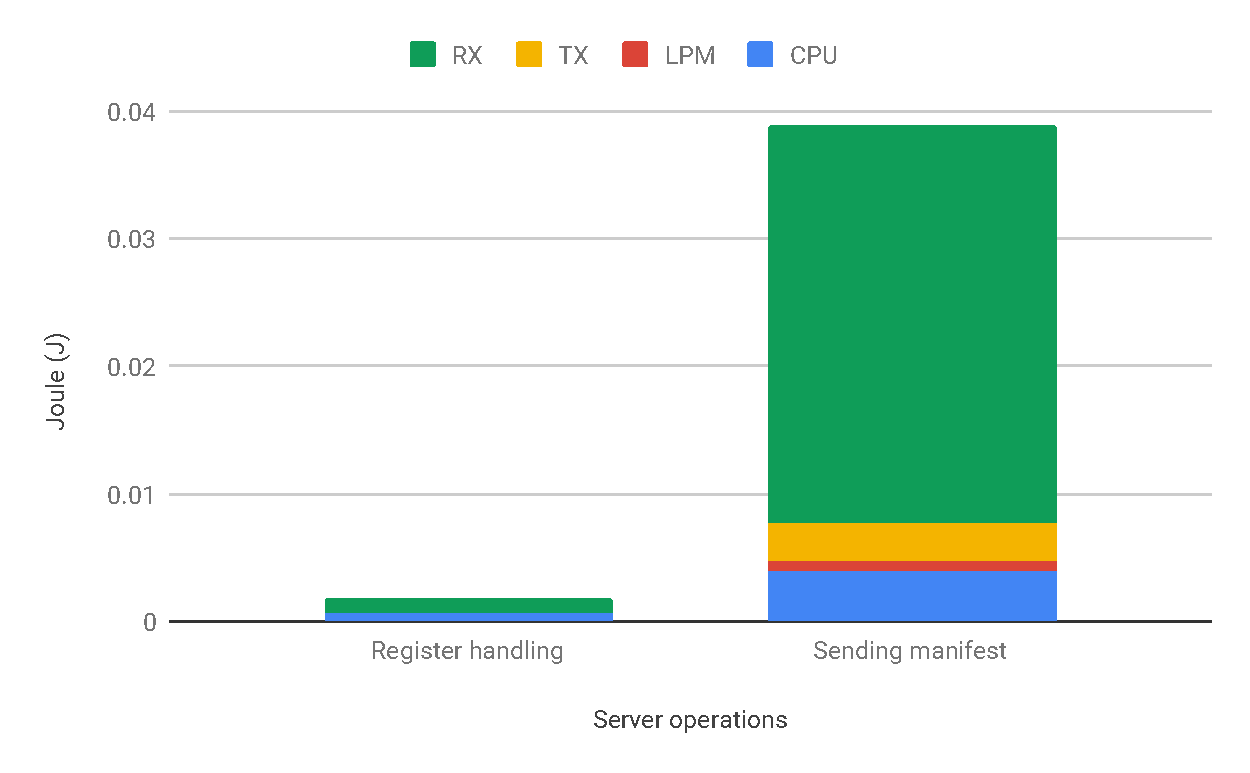
\includegraphics[scale=0.8]{images/server-operations-energy.pdf}
\end{figure}

\begin{figure}
    \caption{Average energy consumption for server operations.}
    \label{fig:server-operations-energy}
    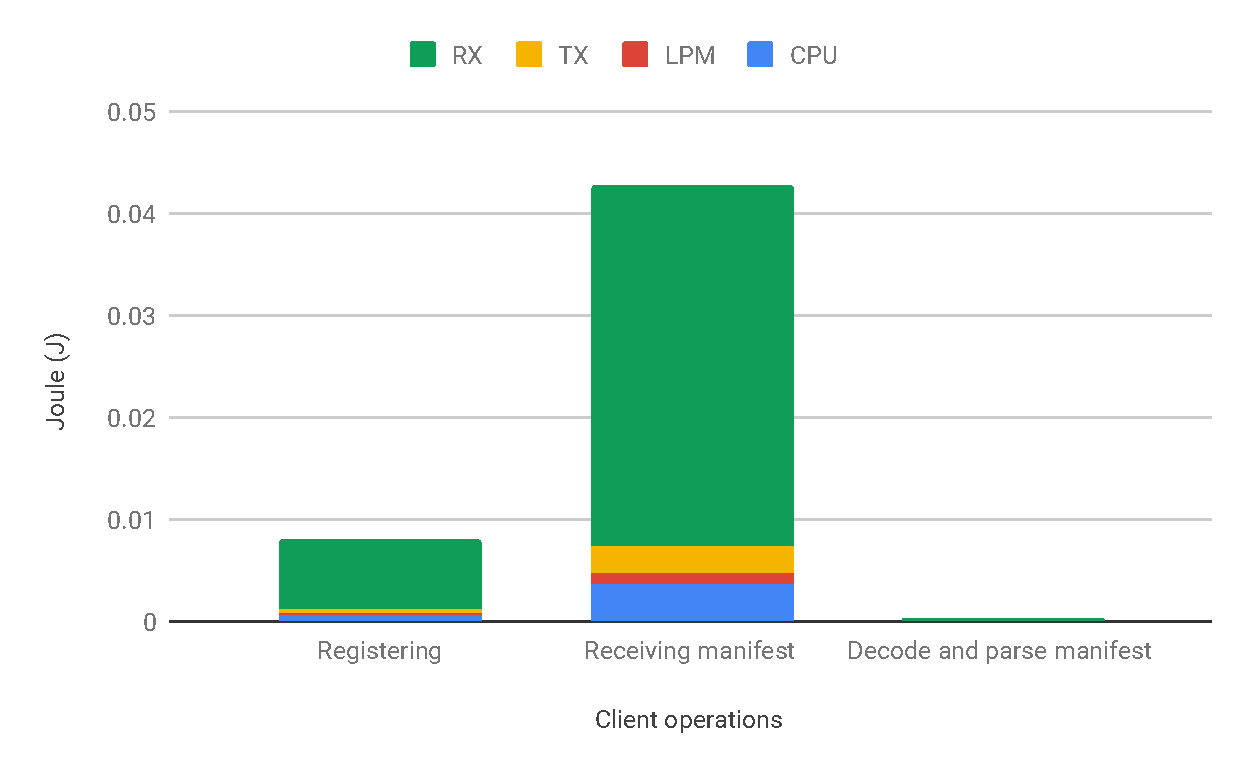
\includegraphics[scale=0.8]{images/client-operations-energy.pdf}
\end{figure}

Figure~\ref{fig:client-image-energy} shows average energy consumption for the client when
retreiving and decrypting image data per block size, ten runs per block size.
Figure~\ref{fig:server-image-energy} shows average energy consumption for the server when
encrypting and sending image data per block size, ten runs per block size.

\begin{figure}
    \caption{Average energy consumption for client during image transfer.}
    \label{fig:client-image-energy}
    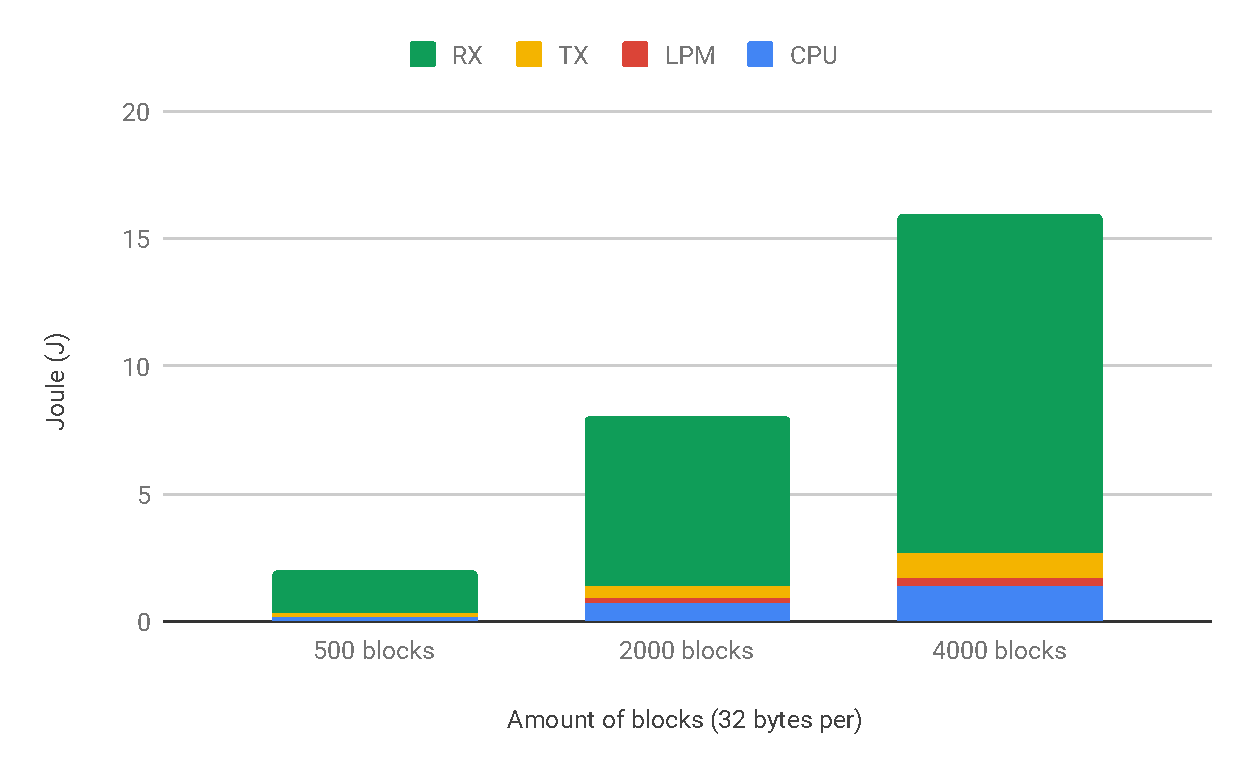
\includegraphics[scale=0.8]{images/client-image-energy.pdf}
\end{figure}

\begin{figure}
    \caption{Average energy consumption for server during image transfer.}
    \label{fig:server-image-energy}
    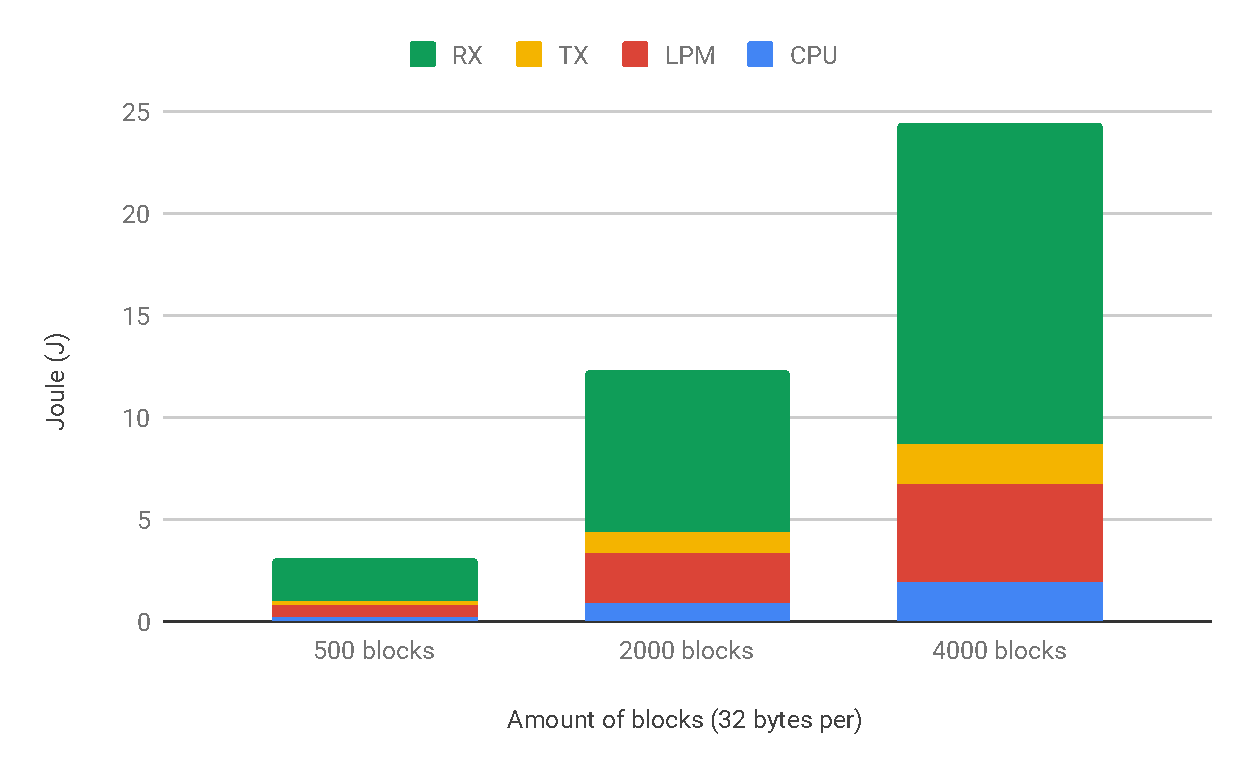
\includegraphics[scale=0.8]{images/server-image-energy.pdf}
\end{figure}

\subsection{Communication Overhead}
\label{ssec:communication-overhead}
Communication overhead of update procedure.
Describe how measurements are obtained (latency and packet size? dont know how to do lossy
stuff)

\subsection{Code Size}
\label{ssec:code-size}
When measuring code size, the code was compiled with all debug macros set to 0 and without
the energest code. By running the tool arm-none-eabi-size on the ELF-files the code size
can be obtained, which is shown in Table~\ref{tab:code-size}.

\begin{table}
\begin{tabular}{l c r r r l}
text	&  data	 &  bss	 &  dec	 &  hex&filename\\
75956	&  1788	 &13599	 &91343	 &164cf&update-client.elf\\
77924	&  1884	 &11835	 &91643	 &165fb&update-server.elf
\end{tabular}
\caption{Code size for client and server prototypes.}
\label{tab:code-size}
\end{table}

\section{Qualitative Evaluation of Update Architecture}
\label{sec:qual-evaluation}
The proposed architecture can be evaluated in two parts analogous to how the SUIT working
group presented their work, namely architecture and information model. Using the
requirements of each document, a qualitative evaluation of the proposed architecture can
be performed. The requirements are gathered from \parencite{suit-architecture,
suit-information-model}.
\subsection{Architecture}
\label{ssec:arch-evaluation}
The SUIT architecture document specified ten requirements a suitable update architecture
should fulfill:

\begin{description}
    \item[Agnostic to how firmware images are distributed:]
        No parts of the architecture assumes a specific suite of protocols or algorithms
        to ensure secure delivery of updates. The architecture does specify the usage of
        technologies such as certificates, asymmetric encryption, and authorization
        tokens, but these elements can be implemented in a wide variety of ways using
        different protocols, algorithms, and certificate/token types. The profiles
        provided in the thesis are examples of how specific incarnations of the
        architecture could look like.

    \item[Friendly to broadcast delivery:]
        The architecture itself does not limit broadcast delivery and through correct
        usage of the manifest broadcasted updates will not be incorrectly installed by
        devices other than the intended recipients. Choice of technology can limit the
        usage of broadcasting, such as DTLS, but this is implementation specific.

    \item[Use state-of-the-art security mechanisms:]
        The architecture is based on asymmetric cryptography using certificates as well as
        access authorization through whitelists and possibly tokens for fine-grain
        authorization. Choice of key algorithms and token types will affect the resilience
        of the system, allowing for both smaller and less strong keys and tokens or larger
        and strong keys and tokens. % TODO: Swap resilience for something like
        % cryptographic strength

    \item[Rollback attacks must be prevented:]
        By specifying a monotonically increasing sequence number in the manifest, devices
        can make sure they are installing fresh images. Manifests are signed through COSE
        which ensures authenticity, an assailant would not be able to modify a manifest
        and then recompute a valid signature.

    \item[High reliability:]
        This is an implementation specific requirement, however the storage element of the
        manifest aids in achieving safe storage of a new image. After a successful update,
        devices are to re-register at servers. No acknowledgment means the server knows
        the update still must be applied, thus an interrupted update can be redistributed.

    \item[Operate with a small bootloader:]
        The thesis suggests to store an unencrypted image alongside its digest for the
        bootloader to be minimal, only needing support for calculating a SHA256 digest of
        the image at boot. All information about whether or not to perform the update is
        encoded in conditions in the manifest, and can be stored with small memory usage.

    \item[Small parsers:]
        The manifest format used in the thesis is simple, complete, and extensible.
        Parsing it requires storing the key/value pairs in predefined structures which is
        possible with a very small parser.

    \item[Minimal impact on existing firmware formats:]
        The architecture makes no assumptions about firmware formats. It is up to the
        implementer to ensure the images are prepared for updating and that the bootloader
        contains the necessary functionality. Transporting the images is the same
        regardless of content.

    \item[Robust permissions:]
        The architecture is based on asymmetric cryptography using certificates for
        identity and confidentiality, and whitelists of servers and operators as well as
        tokens for authorization. Different deployments have different security and
        performance requirements, the architecture is flexible by allowing different kinds
        of key algorithms, encryption schemes, and token types. Some deployments may not
        need tokens at all as authentication is done on a device level and whitelists are
        sufficient, white other deployments wanting to update specific pieces of a device
        may need fine-grained authorization through tokens. Different devices in the same
        deployment can have different authorization configurations, for instance by
        accepting different types of tokens.

    \item[Operating modes:]
        The architecture supports the device initiated pull model as well as the operator
        initiated push model. The update server acts as a mediator between device and
        operator as well as a repository for images and device profiles, letting the
        operator query the server for device statuses and devices query for updates
        depending on the model used.
\end{description}

In addition to these requirements, the architecture discusses the following
topics/introduces the following considerations:
Servers as communication proxies between operator (unconstrained) and device (constrained)
Life cycle approach of enrolling and re-enrolling in an update architecture
Defined the notion of operators, update servers, and devices
Profiles have been developed and one profile implemented in a prototype (with some
constraints such as certificates and tokens)

% TODO: Add anything the architecture might have contributed with (device
% profiles/communication/targeting of updates, definitions of operators and update servers)
  
\subsection{Information Model}
\label{ssec:information-evaluation}
The information model had more requirements posed upon it than the architecture and its
implementation forms an important basis for carrying out safe updates. Evaluating the
proposed manifest format and implementation against the requirements of the specification
yields the following:

\begin{description}
    \item[Installation instructions:]
        Installation instructions or any sort of directive is not included in the base
        manifest structure but can be implemented in the options field. Directives, shown
        as an option in Figure~\ref{fig:manifest-format}, could be used to indicate
        decompression algorithms, preparation of bootloader etc while other more specific
        instructions can be implemented either as a directive or a new kind of option
        element specific to that deployment.

    \item[Override non-critical manifest elements:]
        The proposed manifest format has the critical elements as a baseline and the rest
        severed into the options field. Defining new option types allows for new
        elements in the manifest, but the devices need to be updated for their parsers and
        manifest checkers to be aware of the new elements.

    \item[Modular update:]
        Supported through precursor images, dependencies, URI aliases, and the use of
        authorization tokens for more granular updates. For devices with several MCUs and
        applications, possibly several operating systems, update access can be controlled
        through authorization tokens such that a vendor can only update their respective
        part.

    \item[Multiple authorizations:]
        Enforced via operator and update server whitelists and authorization tokens.

    \item[Multiple payload formats:]
        The architecture and manifest format does not make assumptions about the payload
        formats. The mappings of formats to keys in the manifest is deployment
        specific and whatever formats a deployment might opt to use can be represented in
        the manifest together with a SHA256 digest of said format.

    \item[Prevent confidential information disclosure:]
        The architecture is based on state-of-the-art security mechanisms and achieves
        confidentiality through asymmetric cryptography. Both manifest and payload are
        encrypted and then signed using COSE.

    \item[Prevent devices from unpacking unknown formats:]
        Supported through the use of the manifest format element, preconditions,
        overridable/custom directives, and letting the update server decide if there is a
        suitable update for a device by matching against its registered profile.

    \item[Specify version numbers of target firmware:]
        Since devices are required to register their version alongside vendor and class
        ID, operators can query device statutes from the update server and then prepare
        updates matching these categories of devices.

    \item[Enable devices to choose between images:]
        Several images can be specified in a single manifest through the use of either
        precursors, dependencies, URIs (mirror list), or aliases depending on the specific
        use case. New options can also be defined capturing this behaviour, such as a new
        option providing URL/Digest pairs intended for parallel storage.

    \item[Secure boot using manifests:]
        The thesis has not examined bootloaders, thus this requirement is out of scope.
        Investigating secure bootloaders could be part of future work in the topic.

    \item[Decompress on load:]
        This behaviour can be encoded in the payload format of the manifest, or through
        the use of a custom directive indicating a compressed payload is stored.

    \item[Payload in manifest:]
        Can be added as the optional "payload" element, the value would be the data of the
        payload and the regular payloadInfo element would contain its digest. Worth noting
        is that for most deployments including the payload in the manifest will
        dramatically increase the size of manifest, thus a manifest parser must be
        prepared for it.

    \item[Simple parsing:]
        As explained in the previous section, the manifest format is simple and easy to
        parse even for constrained devices.
\end{description}

\section{Discussion}
\label{sec:discussion}


\subsection{Security Considerations}
\label{ssec:security-considerations}
Despite being able to add timestamps in the manifest specifying a time of update it can
prove difficult to install updates at the right moment. This is especially important for
devices used in safety critical contexts such as in factories. Timestamps are also unable
to account for if processes are being interrupted or not, one might want to postpone
updates until a certain process or thread is idle. The architecture does also not account
for scenarios where redundant devices are used to achieve the same goal, such as
monitoring equipment. To update one of the devices while the other operates and then
update the other would require manual intervention such as sending the devices updates one
at a time.

The architecture does not account for physical threats, only threats that arise during
wireless transport. The discussion in Section~\ref{ssec:upgrading} does not account for
scenarios where the physical storage of devices is compromised. Implementers are advised
to store manifest and image data in a way that makes sense for their own deployment,
whether that is unencrypted, encrypted, or encrypted manifest with unencrypted image.


\section{Future Work}
\label{sec:future-work}
Moving forward, developing a prototype using certificates instead of pre-shared DTLS keys,
authorization tokens, and COSE signing instead of encryption would further aid the
understanding of the architectures requirements on devices and how feasible it is to use
for less constrained devices. If using Contiki-NG this would require some development work
as none of the mentioned features exist in the operating system at time of writing.
Furthermore, research about bootloaders, safe boot, and storage of firmware images is of
interest as this thesis only covers transportation. How to upgrade a device, how to
perform differential updates, and possibly how to update safety critical systems are all
important topics that can utilize the proposed transport architecture and prototype as a
starting point.

\end{document}